\documentclass[twoside]{book}

% Packages required by doxygen
\usepackage{fixltx2e}
\usepackage{calc}
\usepackage{doxygen}
\usepackage{graphicx}
\usepackage[utf8]{inputenc}
\usepackage{makeidx}
\usepackage{multicol}
\usepackage{multirow}
\PassOptionsToPackage{warn}{textcomp}
\usepackage{textcomp}
\usepackage[nointegrals]{wasysym}
\usepackage[table]{xcolor}

% Font selection
\usepackage[T1]{fontenc}
\usepackage{mathptmx}
\usepackage[scaled=.90]{helvet}
\usepackage{courier}
\usepackage{amssymb}
\usepackage{sectsty}
\renewcommand{\familydefault}{\sfdefault}
\allsectionsfont{%
  \fontseries{bc}\selectfont%
  \color{darkgray}%
}
\renewcommand{\DoxyLabelFont}{%
  \fontseries{bc}\selectfont%
  \color{darkgray}%
}
\newcommand{\+}{\discretionary{\mbox{\scriptsize$\hookleftarrow$}}{}{}}

% Page & text layout
\usepackage{geometry}
\geometry{%
  a4paper,%
  top=2.5cm,%
  bottom=2.5cm,%
  left=2.5cm,%
  right=2.5cm%
}
\tolerance=750
\hfuzz=15pt
\hbadness=750
\setlength{\emergencystretch}{15pt}
\setlength{\parindent}{0cm}
\setlength{\parskip}{0.2cm}
\makeatletter
\renewcommand{\paragraph}{%
  \@startsection{paragraph}{4}{0ex}{-1.0ex}{1.0ex}{%
    \normalfont\normalsize\bfseries\SS@parafont%
  }%
}
\renewcommand{\subparagraph}{%
  \@startsection{subparagraph}{5}{0ex}{-1.0ex}{1.0ex}{%
    \normalfont\normalsize\bfseries\SS@subparafont%
  }%
}
\makeatother

% Headers & footers
\usepackage{fancyhdr}
\pagestyle{fancyplain}
\fancyhead[LE]{\fancyplain{}{\bfseries\thepage}}
\fancyhead[CE]{\fancyplain{}{}}
\fancyhead[RE]{\fancyplain{}{\bfseries\leftmark}}
\fancyhead[LO]{\fancyplain{}{\bfseries\rightmark}}
\fancyhead[CO]{\fancyplain{}{}}
\fancyhead[RO]{\fancyplain{}{\bfseries\thepage}}
\fancyfoot[LE]{\fancyplain{}{}}
\fancyfoot[CE]{\fancyplain{}{}}
\fancyfoot[RE]{\fancyplain{}{\bfseries\scriptsize Generated on Wed Nov 2 2016 22\+:39\+:21 for Lab5 by Doxygen }}
\fancyfoot[LO]{\fancyplain{}{\bfseries\scriptsize Generated on Wed Nov 2 2016 22\+:39\+:21 for Lab5 by Doxygen }}
\fancyfoot[CO]{\fancyplain{}{}}
\fancyfoot[RO]{\fancyplain{}{}}
\renewcommand{\footrulewidth}{0.4pt}
\renewcommand{\chaptermark}[1]{%
  \markboth{#1}{}%
}
\renewcommand{\sectionmark}[1]{%
  \markright{\thesection\ #1}%
}

% Indices & bibliography
\usepackage{natbib}
\usepackage[titles]{tocloft}
\setcounter{tocdepth}{3}
\setcounter{secnumdepth}{5}
\makeindex

% Hyperlinks (required, but should be loaded last)
\usepackage{ifpdf}
\ifpdf
  \usepackage[pdftex,pagebackref=true]{hyperref}
\else
  \usepackage[ps2pdf,pagebackref=true]{hyperref}
\fi
\hypersetup{%
  colorlinks=true,%
  linkcolor=blue,%
  citecolor=blue,%
  unicode%
}

% Custom commands
\newcommand{\clearemptydoublepage}{%
  \newpage{\pagestyle{empty}\cleardoublepage}%
}


%===== C O N T E N T S =====

\begin{document}

% Titlepage & ToC
\hypersetup{pageanchor=false,
             bookmarks=true,
             bookmarksnumbered=true,
             pdfencoding=unicode
            }
\pagenumbering{roman}
\begin{titlepage}
\vspace*{7cm}
\begin{center}%
{\Large Lab5 }\\
\vspace*{1cm}
{\large Generated by Doxygen 1.8.8}\\
\vspace*{0.5cm}
{\small Wed Nov 2 2016 22:39:21}\\
\end{center}
\end{titlepage}
\clearemptydoublepage
\tableofcontents
\clearemptydoublepage
\pagenumbering{arabic}
\hypersetup{pageanchor=true}

%--- Begin generated contents ---
\chapter{Hierarchical Index}
\section{Class Hierarchy}
This inheritance list is sorted roughly, but not completely, alphabetically\+:\begin{DoxyCompactList}
\item \contentsline{section}{Carta}{\pageref{class_carta}}{}
\item \contentsline{section}{Celda$<$ T $>$}{\pageref{class_celda}}{}
\item \contentsline{section}{Jugador}{\pageref{class_jugador}}{}
\item \contentsline{section}{Lista$<$ T $>$}{\pageref{class_lista}}{}
\begin{DoxyCompactList}
\item \contentsline{section}{Lista\+Con\+Arreglo$<$ T $>$}{\pageref{class_lista_con_arreglo}}{}
\item \contentsline{section}{Lista\+Con\+Puntero$<$ T $>$}{\pageref{class_lista_con_puntero}}{}
\end{DoxyCompactList}
\item \contentsline{section}{Lista$<$ char $>$}{\pageref{class_lista}}{}
\begin{DoxyCompactList}
\item \contentsline{section}{Lista\+Con\+Arreglo$<$ char $>$}{\pageref{class_lista_con_arreglo}}{}
\end{DoxyCompactList}
\item \contentsline{section}{Mazo}{\pageref{class_mazo}}{}
\item \contentsline{section}{Mesa}{\pageref{class_mesa}}{}
\item \contentsline{section}{Portero}{\pageref{class_portero}}{}
\end{DoxyCompactList}

\chapter{Class Index}
\section{Class List}
Here are the classes, structs, unions and interfaces with brief descriptions\+:\begin{DoxyCompactList}
\item\contentsline{section}{\hyperlink{class_juego_de_la_vida}{Juego\+De\+La\+Vida} }{\pageref{class_juego_de_la_vida}}{}
\end{DoxyCompactList}

\chapter{Class Documentation}
\hypertarget{class_carta}{\section{Carta Class Reference}
\label{class_carta}\index{Carta@{Carta}}
}


Collaboration diagram for Carta\+:
\nopagebreak
\begin{figure}[H]
\begin{center}
\leavevmode
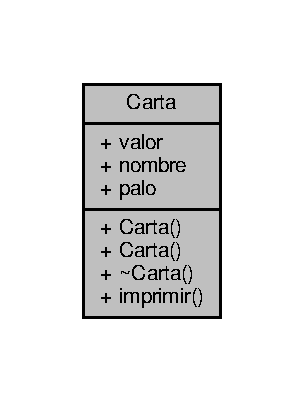
\includegraphics[width=146pt]{class_carta__coll__graph}
\end{center}
\end{figure}
\subsection*{Public Member Functions}
\begin{DoxyCompactItemize}
\item 
\hypertarget{class_carta_a769e6bdb8d3725177481b32e4dbbbd66}{\hyperlink{class_carta_a769e6bdb8d3725177481b32e4dbbbd66}{Carta} ()}\label{class_carta_a769e6bdb8d3725177481b32e4dbbbd66}

\begin{DoxyCompactList}\small\item\em Constructores y destructores de \hyperlink{class_carta}{Carta}. \end{DoxyCompactList}\item 
\hypertarget{class_carta_a3b344c050b8fc2fdf04caf9577bdeda5}{{\bfseries Carta} (int \hyperlink{class_carta_a40ed698935c3b770a0b118dea14c667b}{valor}, string nombre, string palo)}\label{class_carta_a3b344c050b8fc2fdf04caf9577bdeda5}

\item 
\hypertarget{class_carta_a9a8f66923d83b66bf20289dc6e07874f}{void \hyperlink{class_carta_a9a8f66923d83b66bf20289dc6e07874f}{imprimir} ()}\label{class_carta_a9a8f66923d83b66bf20289dc6e07874f}

\begin{DoxyCompactList}\small\item\em Funciones de \hyperlink{class_carta}{Carta}. \end{DoxyCompactList}\end{DoxyCompactItemize}
\subsection*{Public Attributes}
\begin{DoxyCompactItemize}
\item 
\hypertarget{class_carta_a40ed698935c3b770a0b118dea14c667b}{int \hyperlink{class_carta_a40ed698935c3b770a0b118dea14c667b}{valor}}\label{class_carta_a40ed698935c3b770a0b118dea14c667b}

\begin{DoxyCompactList}\small\item\em Atributos de \hyperlink{class_carta}{Carta}. \end{DoxyCompactList}\item 
\hypertarget{class_carta_af9ecddff3f4ac2ffe4a00a5ec62a3b29}{string {\bfseries nombre}}\label{class_carta_af9ecddff3f4ac2ffe4a00a5ec62a3b29}

\item 
\hypertarget{class_carta_a708b56ce311c1ea2329a76c60d740881}{string {\bfseries palo}}\label{class_carta_a708b56ce311c1ea2329a76c60d740881}

\end{DoxyCompactItemize}


The documentation for this class was generated from the following files\+:\begin{DoxyCompactItemize}
\item 
Carta.\+h\item 
Carta.\+cpp\end{DoxyCompactItemize}

\hypertarget{class_celda}{\section{Celda$<$ T $>$ Class Template Reference}
\label{class_celda}\index{Celda$<$ T $>$@{Celda$<$ T $>$}}
}


Collaboration diagram for Celda$<$ T $>$\+:
\nopagebreak
\begin{figure}[H]
\begin{center}
\leavevmode
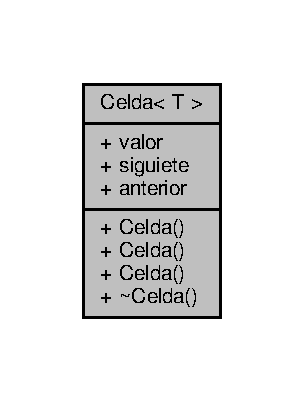
\includegraphics[width=146pt]{class_celda__coll__graph}
\end{center}
\end{figure}
\subsection*{Public Member Functions}
\begin{DoxyCompactItemize}
\item 
\hypertarget{class_celda_a19d4004458f354c8aef4145e9135b58d}{{\bfseries Celda} (T valor)}\label{class_celda_a19d4004458f354c8aef4145e9135b58d}

\item 
\hypertarget{class_celda_a63648973285cd58a2ea2fb5bf47a0aeb}{{\bfseries Celda} (const \hyperlink{class_celda}{Celda} \&orig)}\label{class_celda_a63648973285cd58a2ea2fb5bf47a0aeb}

\end{DoxyCompactItemize}
\subsection*{Public Attributes}
\begin{DoxyCompactItemize}
\item 
\hypertarget{class_celda_a4165d991b55ff069ebc6019b03c8463d}{T {\bfseries valor}}\label{class_celda_a4165d991b55ff069ebc6019b03c8463d}

\item 
\hypertarget{class_celda_a5ad2ff91a15992430a17af7d6431f3a0}{\hyperlink{class_celda}{Celda}$<$ T $>$ $\ast$ {\bfseries siguiete}}\label{class_celda_a5ad2ff91a15992430a17af7d6431f3a0}

\item 
\hypertarget{class_celda_aacbb2f1f4e4fad69db9ae11c18b02382}{\hyperlink{class_celda}{Celda}$<$ T $>$ $\ast$ {\bfseries anterior}}\label{class_celda_aacbb2f1f4e4fad69db9ae11c18b02382}

\end{DoxyCompactItemize}


The documentation for this class was generated from the following file\+:\begin{DoxyCompactItemize}
\item 
Celda.\+h\end{DoxyCompactItemize}

\hypertarget{class_jugador}{\section{Jugador Class Reference}
\label{class_jugador}\index{Jugador@{Jugador}}
}


Collaboration diagram for Jugador\+:
\nopagebreak
\begin{figure}[H]
\begin{center}
\leavevmode
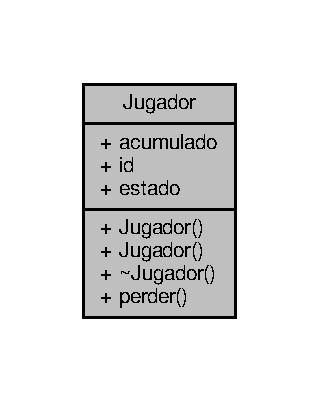
\includegraphics[width=153pt]{class_jugador__coll__graph}
\end{center}
\end{figure}
\subsection*{Public Member Functions}
\begin{DoxyCompactItemize}
\item 
\hypertarget{class_jugador_a232c46f75691af6210096e5972535d71}{\hyperlink{class_jugador_a232c46f75691af6210096e5972535d71}{Jugador} ()}\label{class_jugador_a232c46f75691af6210096e5972535d71}

\begin{DoxyCompactList}\small\item\em Constructor vacío de \hyperlink{class_jugador}{Jugador}. \end{DoxyCompactList}\item 
\hypertarget{class_jugador_ac3ba0a32d09db7367efe4cd9e019e41d}{\hyperlink{class_jugador_ac3ba0a32d09db7367efe4cd9e019e41d}{Jugador} (char id)}\label{class_jugador_ac3ba0a32d09db7367efe4cd9e019e41d}

\begin{DoxyCompactList}\small\item\em Constructor de \hyperlink{class_jugador}{Jugador}. \end{DoxyCompactList}\item 
\hypertarget{class_jugador_a9db1d422fe3b675f92d9fd687b1f42c4}{virtual \hyperlink{class_jugador_a9db1d422fe3b675f92d9fd687b1f42c4}{$\sim$\+Jugador} ()}\label{class_jugador_a9db1d422fe3b675f92d9fd687b1f42c4}

\begin{DoxyCompactList}\small\item\em Destructor de \hyperlink{class_portero}{Portero}. \end{DoxyCompactList}\item 
\hypertarget{class_jugador_ad483ad724147364ee91a822f471c09b2}{void \hyperlink{class_jugador_ad483ad724147364ee91a822f471c09b2}{perder} ()}\label{class_jugador_ad483ad724147364ee91a822f471c09b2}

\begin{DoxyCompactList}\small\item\em Función cuando un jugador pierde. \end{DoxyCompactList}\end{DoxyCompactItemize}
\subsection*{Public Attributes}
\begin{DoxyCompactItemize}
\item 
\hypertarget{class_jugador_a9df72c40dc67cb49d963bfa756376546}{int \hyperlink{class_jugador_a9df72c40dc67cb49d963bfa756376546}{acumulado}}\label{class_jugador_a9df72c40dc67cb49d963bfa756376546}

\begin{DoxyCompactList}\small\item\em Atributos del Potero. \end{DoxyCompactList}\item 
\hypertarget{class_jugador_a7b805ffc7559ea34bddcb80564832a39}{char {\bfseries id}}\label{class_jugador_a7b805ffc7559ea34bddcb80564832a39}

\item 
\hypertarget{class_jugador_a83b46d72f29a510f670297d55cf9197b}{int {\bfseries estado}}\label{class_jugador_a83b46d72f29a510f670297d55cf9197b}

\end{DoxyCompactItemize}


The documentation for this class was generated from the following files\+:\begin{DoxyCompactItemize}
\item 
Jugador.\+h\item 
Jugador.\+cpp\end{DoxyCompactItemize}

\hypertarget{class_lista}{\section{Lista$<$ T $>$ Class Template Reference}
\label{class_lista}\index{Lista$<$ T $>$@{Lista$<$ T $>$}}
}


Inheritance diagram for Lista$<$ T $>$\+:
\nopagebreak
\begin{figure}[H]
\begin{center}
\leavevmode
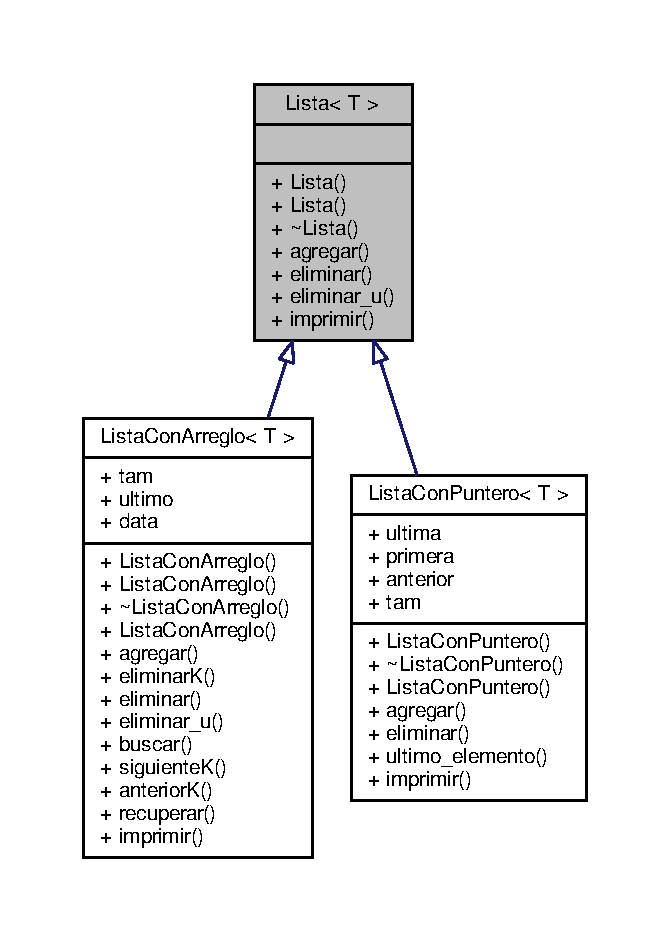
\includegraphics[width=322pt]{class_lista__inherit__graph}
\end{center}
\end{figure}


Collaboration diagram for Lista$<$ T $>$\+:
\nopagebreak
\begin{figure}[H]
\begin{center}
\leavevmode
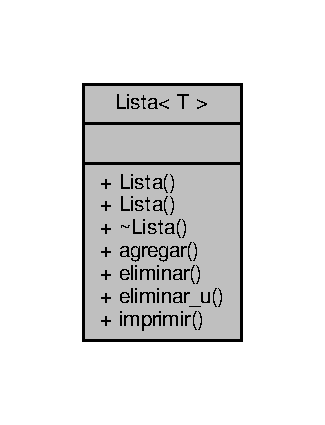
\includegraphics[width=156pt]{class_lista__coll__graph}
\end{center}
\end{figure}
\subsection*{Public Member Functions}
\begin{DoxyCompactItemize}
\item 
\hypertarget{class_lista_ad63a49df32595e2f321fffd7ffa1346a}{{\bfseries Lista} (const \hyperlink{class_lista}{Lista} \&orig)}\label{class_lista_ad63a49df32595e2f321fffd7ffa1346a}

\item 
\hypertarget{class_lista_aea57814c283f14cd0d31b8da37c622a9}{virtual void {\bfseries agregar} (T e)=0}\label{class_lista_aea57814c283f14cd0d31b8da37c622a9}

\item 
\hypertarget{class_lista_aabdd833f1bc38b8174838f92c5b438b3}{virtual void {\bfseries eliminar} ()=0}\label{class_lista_aabdd833f1bc38b8174838f92c5b438b3}

\item 
\hypertarget{class_lista_aa0da522793d55d38f5ba1faf4354b1df}{virtual void {\bfseries eliminar\+\_\+u} ()=0}\label{class_lista_aa0da522793d55d38f5ba1faf4354b1df}

\item 
\hypertarget{class_lista_af398229330911af031fc1d89a556a840}{virtual void {\bfseries imprimir} ()=0}\label{class_lista_af398229330911af031fc1d89a556a840}

\end{DoxyCompactItemize}


The documentation for this class was generated from the following file\+:\begin{DoxyCompactItemize}
\item 
Lista.\+h\end{DoxyCompactItemize}

\hypertarget{class_lista_con_arreglo}{\section{Lista\+Con\+Arreglo$<$ T $>$ Class Template Reference}
\label{class_lista_con_arreglo}\index{Lista\+Con\+Arreglo$<$ T $>$@{Lista\+Con\+Arreglo$<$ T $>$}}
}


Inheritance diagram for Lista\+Con\+Arreglo$<$ T $>$\+:
\nopagebreak
\begin{figure}[H]
\begin{center}
\leavevmode
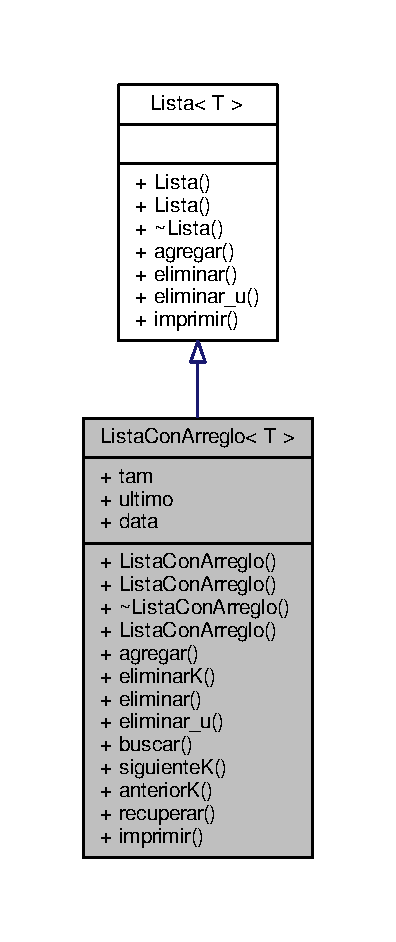
\includegraphics[width=190pt]{class_lista_con_arreglo__inherit__graph}
\end{center}
\end{figure}


Collaboration diagram for Lista\+Con\+Arreglo$<$ T $>$\+:
\nopagebreak
\begin{figure}[H]
\begin{center}
\leavevmode
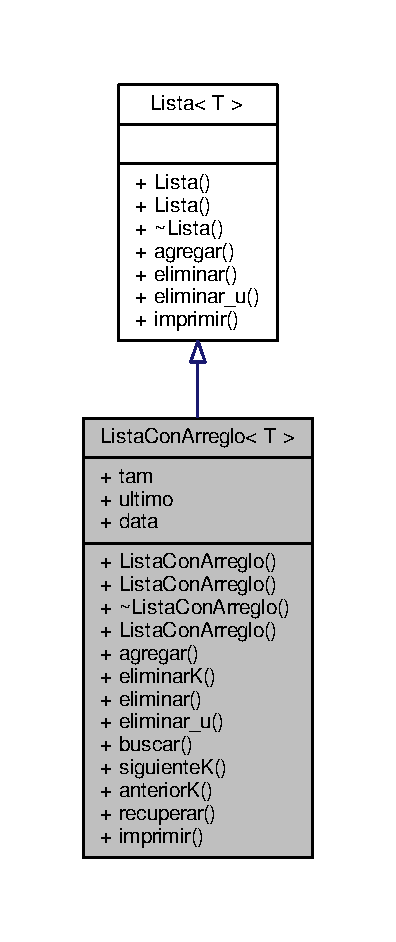
\includegraphics[width=190pt]{class_lista_con_arreglo__coll__graph}
\end{center}
\end{figure}
\subsection*{Public Member Functions}
\begin{DoxyCompactItemize}
\item 
\hypertarget{class_lista_con_arreglo_ab7a22a8f04de9403d32a7431d4dd9627}{{\bfseries Lista\+Con\+Arreglo} (const \hyperlink{class_lista_con_arreglo}{Lista\+Con\+Arreglo} \&orig)}\label{class_lista_con_arreglo_ab7a22a8f04de9403d32a7431d4dd9627}

\item 
\hypertarget{class_lista_con_arreglo_a9541812a0019b76c6529184356913a59}{{\bfseries Lista\+Con\+Arreglo} (int N)}\label{class_lista_con_arreglo_a9541812a0019b76c6529184356913a59}

\item 
\hypertarget{class_lista_con_arreglo_a5336f6ef59e2cfaa008c4ad8cbee9f25}{void {\bfseries agregar} (T e)}\label{class_lista_con_arreglo_a5336f6ef59e2cfaa008c4ad8cbee9f25}

\item 
\hypertarget{class_lista_con_arreglo_acd8b8f484dc440dc64dc58cad375e7e4}{void {\bfseries eliminar\+K} (int k)}\label{class_lista_con_arreglo_acd8b8f484dc440dc64dc58cad375e7e4}

\item 
\hypertarget{class_lista_con_arreglo_a1d4ea3c3bbefa8d2c12ea520e12f5f9c}{virtual void {\bfseries eliminar} ()}\label{class_lista_con_arreglo_a1d4ea3c3bbefa8d2c12ea520e12f5f9c}

\item 
\hypertarget{class_lista_con_arreglo_a9f0f4138dcf42e664213ffbcedce2056}{virtual void {\bfseries eliminar\+\_\+u} ()}\label{class_lista_con_arreglo_a9f0f4138dcf42e664213ffbcedce2056}

\item 
\hypertarget{class_lista_con_arreglo_af2fe968f5ec674cb9640e11a1bcaab99}{int {\bfseries buscar} (T e)}\label{class_lista_con_arreglo_af2fe968f5ec674cb9640e11a1bcaab99}

\item 
\hypertarget{class_lista_con_arreglo_a8a3d5d83291eeab7d9dbb2108a6942ea}{char {\bfseries siguiente\+K} (int k)}\label{class_lista_con_arreglo_a8a3d5d83291eeab7d9dbb2108a6942ea}

\item 
\hypertarget{class_lista_con_arreglo_a78e25313648f0d4f188f61f60d7ba4b6}{char {\bfseries anterior\+K} (int k)}\label{class_lista_con_arreglo_a78e25313648f0d4f188f61f60d7ba4b6}

\item 
\hypertarget{class_lista_con_arreglo_af880c9a6795cf9281f2a217d0a4b0c07}{T {\bfseries recuperar} (int k)}\label{class_lista_con_arreglo_af880c9a6795cf9281f2a217d0a4b0c07}

\item 
\hypertarget{class_lista_con_arreglo_aa8267cef7510ef79626a812b3c85505d}{void {\bfseries imprimir} ()}\label{class_lista_con_arreglo_aa8267cef7510ef79626a812b3c85505d}

\end{DoxyCompactItemize}
\subsection*{Public Attributes}
\begin{DoxyCompactItemize}
\item 
\hypertarget{class_lista_con_arreglo_a7b1a9c6334db75f4ffb023a95b01e3f4}{int {\bfseries tam}}\label{class_lista_con_arreglo_a7b1a9c6334db75f4ffb023a95b01e3f4}

\item 
\hypertarget{class_lista_con_arreglo_a41f052fbde3598cb6f7ec7d8412be8c3}{int {\bfseries ultimo}}\label{class_lista_con_arreglo_a41f052fbde3598cb6f7ec7d8412be8c3}

\item 
\hypertarget{class_lista_con_arreglo_af5771ddbfd5f2fbd5925cb5bae26908e}{T $\ast$ {\bfseries data}}\label{class_lista_con_arreglo_af5771ddbfd5f2fbd5925cb5bae26908e}

\end{DoxyCompactItemize}


The documentation for this class was generated from the following file\+:\begin{DoxyCompactItemize}
\item 
Lista\+Con\+Arreglo.\+h\end{DoxyCompactItemize}

\hypertarget{class_lista_con_puntero}{\section{Lista\+Con\+Puntero$<$ T $>$ Class Template Reference}
\label{class_lista_con_puntero}\index{Lista\+Con\+Puntero$<$ T $>$@{Lista\+Con\+Puntero$<$ T $>$}}
}


Inheritance diagram for Lista\+Con\+Puntero$<$ T $>$\+:
\nopagebreak
\begin{figure}[H]
\begin{center}
\leavevmode
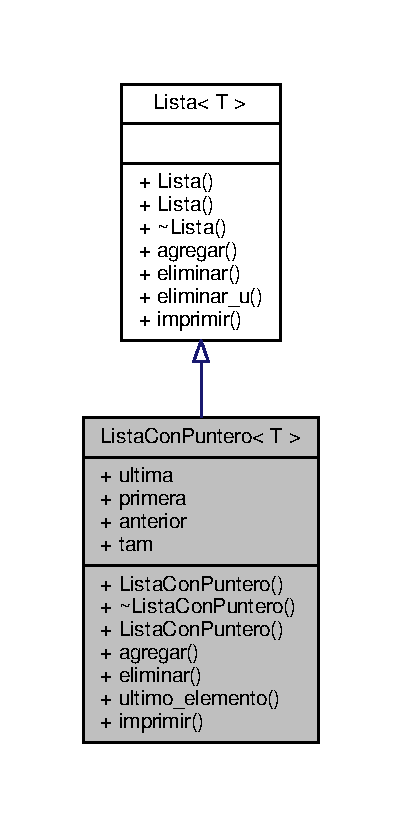
\includegraphics[width=193pt]{class_lista_con_puntero__inherit__graph}
\end{center}
\end{figure}


Collaboration diagram for Lista\+Con\+Puntero$<$ T $>$\+:
\nopagebreak
\begin{figure}[H]
\begin{center}
\leavevmode
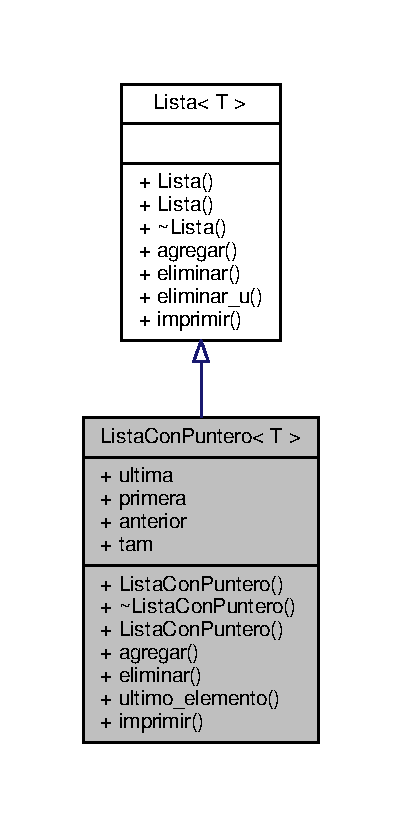
\includegraphics[width=193pt]{class_lista_con_puntero__coll__graph}
\end{center}
\end{figure}
\subsection*{Public Member Functions}
\begin{DoxyCompactItemize}
\item 
\hypertarget{class_lista_con_puntero_ae7de4e8c809b2b2e3f5ded5279f4cb13}{{\bfseries Lista\+Con\+Puntero} (const \hyperlink{class_lista_con_puntero}{Lista\+Con\+Puntero} \&orig)}\label{class_lista_con_puntero_ae7de4e8c809b2b2e3f5ded5279f4cb13}

\item 
\hypertarget{class_lista_con_puntero_a22c72f33bd09f3e8f4df32949add7b5a}{{\bfseries Lista\+Con\+Puntero} (int N)}\label{class_lista_con_puntero_a22c72f33bd09f3e8f4df32949add7b5a}

\item 
\hypertarget{class_lista_con_puntero_afc679c900335d45da5f47e5742fc75fa}{void {\bfseries agregar} (T e)}\label{class_lista_con_puntero_afc679c900335d45da5f47e5742fc75fa}

\item 
\hypertarget{class_lista_con_puntero_ab305edeecf878b5c3711a6a59c9622eb}{virtual void {\bfseries eliminar} ()}\label{class_lista_con_puntero_ab305edeecf878b5c3711a6a59c9622eb}

\item 
\hypertarget{class_lista_con_puntero_a0e5d388bf9d8ebcfd52eb470939d51c3}{T {\bfseries ultimo\+\_\+elemento} ()}\label{class_lista_con_puntero_a0e5d388bf9d8ebcfd52eb470939d51c3}

\item 
\hypertarget{class_lista_con_puntero_a99b8e8cfa4c23b07a9a35a55034827fb}{void {\bfseries imprimir} ()}\label{class_lista_con_puntero_a99b8e8cfa4c23b07a9a35a55034827fb}

\end{DoxyCompactItemize}
\subsection*{Public Attributes}
\begin{DoxyCompactItemize}
\item 
\hypertarget{class_lista_con_puntero_abaaf8a6d544bb5762779a186886fce82}{\hyperlink{class_celda}{Celda}$<$ T $>$ $\ast$ {\bfseries ultima}}\label{class_lista_con_puntero_abaaf8a6d544bb5762779a186886fce82}

\item 
\hypertarget{class_lista_con_puntero_a46fe3edc08709d0821ed9d31a64d3ba0}{\hyperlink{class_celda}{Celda}$<$ T $>$ $\ast$ {\bfseries primera}}\label{class_lista_con_puntero_a46fe3edc08709d0821ed9d31a64d3ba0}

\item 
\hypertarget{class_lista_con_puntero_a38e52dfa7b49be4374147d28703e1226}{\hyperlink{class_celda}{Celda}$<$ T $>$ $\ast$ {\bfseries anterior}}\label{class_lista_con_puntero_a38e52dfa7b49be4374147d28703e1226}

\item 
\hypertarget{class_lista_con_puntero_a55db33fa3744c12d51bfadfd85f86dc5}{int {\bfseries tam}}\label{class_lista_con_puntero_a55db33fa3744c12d51bfadfd85f86dc5}

\end{DoxyCompactItemize}


The documentation for this class was generated from the following file\+:\begin{DoxyCompactItemize}
\item 
Lista\+Con\+Puntero.\+h\end{DoxyCompactItemize}

\hypertarget{class_mazo}{\section{Mazo Class Reference}
\label{class_mazo}\index{Mazo@{Mazo}}
}


Collaboration diagram for Mazo\+:
\nopagebreak
\begin{figure}[H]
\begin{center}
\leavevmode
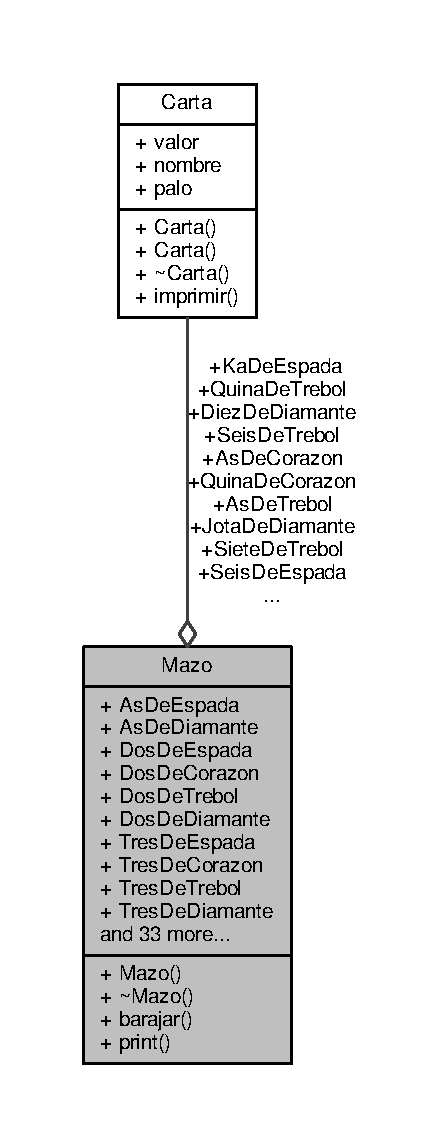
\includegraphics[height=550pt]{class_mazo__coll__graph}
\end{center}
\end{figure}
\subsection*{Public Member Functions}
\begin{DoxyCompactItemize}
\item 
\hypertarget{class_mazo_a93eaa35af9ad42840c3a37d4054ba17d}{\hyperlink{class_mazo_a93eaa35af9ad42840c3a37d4054ba17d}{Mazo} ()}\label{class_mazo_a93eaa35af9ad42840c3a37d4054ba17d}

\begin{DoxyCompactList}\small\item\em Constructor de \hyperlink{class_mazo}{Mazo}. \end{DoxyCompactList}\item 
\hypertarget{class_mazo_a2ce07ca90c706e6454ac54d727d3da2a}{virtual \hyperlink{class_mazo_a2ce07ca90c706e6454ac54d727d3da2a}{$\sim$\+Mazo} ()}\label{class_mazo_a2ce07ca90c706e6454ac54d727d3da2a}

\begin{DoxyCompactList}\small\item\em Destructor de \hyperlink{class_mazo}{Mazo}. \end{DoxyCompactList}\item 
\hypertarget{class_mazo_ad73b15de8ae06e4e7aaecd97626bbe21}{void \hyperlink{class_mazo_ad73b15de8ae06e4e7aaecd97626bbe21}{barajar} ()}\label{class_mazo_ad73b15de8ae06e4e7aaecd97626bbe21}

\begin{DoxyCompactList}\small\item\em Funciones. \end{DoxyCompactList}\item 
\hypertarget{class_mazo_a423b1b45f04d64d2507879b2662deb51}{void {\bfseries print} ()}\label{class_mazo_a423b1b45f04d64d2507879b2662deb51}

\end{DoxyCompactItemize}
\subsection*{Public Attributes}
\begin{DoxyCompactItemize}
\item 
\hypertarget{class_mazo_a6c330982debd67a6c5b34c7564fb22b3}{\hyperlink{class_carta}{Carta} \hyperlink{class_mazo_a6c330982debd67a6c5b34c7564fb22b3}{As\+De\+Espada}}\label{class_mazo_a6c330982debd67a6c5b34c7564fb22b3}

\begin{DoxyCompactList}\small\item\em Atributos. \end{DoxyCompactList}\item 
\hypertarget{class_mazo_a3b3e94f15ab56c2d63449c840dd98966}{\hyperlink{class_carta}{Carta} {\bfseries As\+De\+Corazon}}\label{class_mazo_a3b3e94f15ab56c2d63449c840dd98966}

\item 
\hypertarget{class_mazo_ab01b3678b7bc747a95b63bc8c083fb38}{\hyperlink{class_carta}{Carta} {\bfseries As\+De\+Trebol}}\label{class_mazo_ab01b3678b7bc747a95b63bc8c083fb38}

\item 
\hypertarget{class_mazo_a47439e07305cd6caf88a9de0da36f9c1}{\hyperlink{class_carta}{Carta} {\bfseries As\+De\+Diamante}}\label{class_mazo_a47439e07305cd6caf88a9de0da36f9c1}

\item 
\hypertarget{class_mazo_acb67c41f51532a176f46aa9f37652ac5}{\hyperlink{class_carta}{Carta} {\bfseries Dos\+De\+Espada}}\label{class_mazo_acb67c41f51532a176f46aa9f37652ac5}

\item 
\hypertarget{class_mazo_a7c88deb4b5e3cf25380f96aa18c1600a}{\hyperlink{class_carta}{Carta} {\bfseries Dos\+De\+Corazon}}\label{class_mazo_a7c88deb4b5e3cf25380f96aa18c1600a}

\item 
\hypertarget{class_mazo_af3362c0fcf0ab3810044be61f5cc1693}{\hyperlink{class_carta}{Carta} {\bfseries Dos\+De\+Trebol}}\label{class_mazo_af3362c0fcf0ab3810044be61f5cc1693}

\item 
\hypertarget{class_mazo_ada109c7c8f853e9c90023793dcd90417}{\hyperlink{class_carta}{Carta} {\bfseries Dos\+De\+Diamante}}\label{class_mazo_ada109c7c8f853e9c90023793dcd90417}

\item 
\hypertarget{class_mazo_a494d07be0637862aaf9c9979a0f62aee}{\hyperlink{class_carta}{Carta} {\bfseries Tres\+De\+Espada}}\label{class_mazo_a494d07be0637862aaf9c9979a0f62aee}

\item 
\hypertarget{class_mazo_ae73ae13f4f61d12f976596224ff98e92}{\hyperlink{class_carta}{Carta} {\bfseries Tres\+De\+Corazon}}\label{class_mazo_ae73ae13f4f61d12f976596224ff98e92}

\item 
\hypertarget{class_mazo_a9c608f8b8a32baa2940ef30624be81a2}{\hyperlink{class_carta}{Carta} {\bfseries Tres\+De\+Trebol}}\label{class_mazo_a9c608f8b8a32baa2940ef30624be81a2}

\item 
\hypertarget{class_mazo_a597e56cf6d8b2fb5e52afb0e181cd659}{\hyperlink{class_carta}{Carta} {\bfseries Tres\+De\+Diamante}}\label{class_mazo_a597e56cf6d8b2fb5e52afb0e181cd659}

\item 
\hypertarget{class_mazo_a877035e3bb958c4009201dea533b73ea}{\hyperlink{class_carta}{Carta} {\bfseries Cuatro\+De\+Espada}}\label{class_mazo_a877035e3bb958c4009201dea533b73ea}

\item 
\hypertarget{class_mazo_a5b3c436eaea61eaa1c25078ba06496db}{\hyperlink{class_carta}{Carta} {\bfseries Cuatro\+De\+Corazon}}\label{class_mazo_a5b3c436eaea61eaa1c25078ba06496db}

\item 
\hypertarget{class_mazo_abd05f8bc72267bafd1d7387d93d67651}{\hyperlink{class_carta}{Carta} {\bfseries Cuatro\+De\+Trebol}}\label{class_mazo_abd05f8bc72267bafd1d7387d93d67651}

\item 
\hypertarget{class_mazo_a9c0d70f965b578e3d722769985a9b345}{\hyperlink{class_carta}{Carta} {\bfseries Cuatro\+De\+Diamante}}\label{class_mazo_a9c0d70f965b578e3d722769985a9b345}

\item 
\hypertarget{class_mazo_a8f901356486bcd8caeee703948d184ee}{\hyperlink{class_carta}{Carta} {\bfseries Cinco\+De\+Espada}}\label{class_mazo_a8f901356486bcd8caeee703948d184ee}

\item 
\hypertarget{class_mazo_abfbf78d362288172616186ff357284dc}{\hyperlink{class_carta}{Carta} {\bfseries Cinco\+De\+Corazon}}\label{class_mazo_abfbf78d362288172616186ff357284dc}

\item 
\hypertarget{class_mazo_ab56aba2c57786b2b15b6611de86b302e}{\hyperlink{class_carta}{Carta} {\bfseries Cinco\+De\+Trebol}}\label{class_mazo_ab56aba2c57786b2b15b6611de86b302e}

\item 
\hypertarget{class_mazo_a665cb7ad1125924dbaae74801620d970}{\hyperlink{class_carta}{Carta} {\bfseries Cinco\+De\+Diamante}}\label{class_mazo_a665cb7ad1125924dbaae74801620d970}

\item 
\hypertarget{class_mazo_ab62b9c788e34fb46aa25fccd6d086b52}{\hyperlink{class_carta}{Carta} {\bfseries Seis\+De\+Espada}}\label{class_mazo_ab62b9c788e34fb46aa25fccd6d086b52}

\item 
\hypertarget{class_mazo_af85f5205c11c4243a55a1621354fca86}{\hyperlink{class_carta}{Carta} {\bfseries Seis\+De\+Corazon}}\label{class_mazo_af85f5205c11c4243a55a1621354fca86}

\item 
\hypertarget{class_mazo_a1e518516f5b379c1599313d036ff5095}{\hyperlink{class_carta}{Carta} {\bfseries Seis\+De\+Trebol}}\label{class_mazo_a1e518516f5b379c1599313d036ff5095}

\item 
\hypertarget{class_mazo_af1833d2a43991a09de3b1db7e9425486}{\hyperlink{class_carta}{Carta} {\bfseries Seis\+De\+Diamante}}\label{class_mazo_af1833d2a43991a09de3b1db7e9425486}

\item 
\hypertarget{class_mazo_add889c4d0fa8ba2c61507223593155aa}{\hyperlink{class_carta}{Carta} {\bfseries Siete\+De\+Espada}}\label{class_mazo_add889c4d0fa8ba2c61507223593155aa}

\item 
\hypertarget{class_mazo_aa3b325fd087d030abd2cc2b388003d72}{\hyperlink{class_carta}{Carta} {\bfseries Siete\+De\+Corazon}}\label{class_mazo_aa3b325fd087d030abd2cc2b388003d72}

\item 
\hypertarget{class_mazo_a8abfb48b4a7599d270de5d5ba95db1aa}{\hyperlink{class_carta}{Carta} {\bfseries Siete\+De\+Trebol}}\label{class_mazo_a8abfb48b4a7599d270de5d5ba95db1aa}

\item 
\hypertarget{class_mazo_a746684bef1afc0f3dfd52dabdb6821ae}{\hyperlink{class_carta}{Carta} {\bfseries Siete\+De\+Diamante}}\label{class_mazo_a746684bef1afc0f3dfd52dabdb6821ae}

\item 
\hypertarget{class_mazo_a618942fe29ab5930954b0e406be0845f}{\hyperlink{class_carta}{Carta} {\bfseries Ocho\+De\+Espada}}\label{class_mazo_a618942fe29ab5930954b0e406be0845f}

\item 
\hypertarget{class_mazo_ab89db4b5e23bcb6dd25f70fc1e878158}{\hyperlink{class_carta}{Carta} {\bfseries Ocho\+De\+Corazon}}\label{class_mazo_ab89db4b5e23bcb6dd25f70fc1e878158}

\item 
\hypertarget{class_mazo_a85d36ed8cfc2acd6afb0ca5cd9bd208e}{\hyperlink{class_carta}{Carta} {\bfseries Ocho\+De\+Trebol}}\label{class_mazo_a85d36ed8cfc2acd6afb0ca5cd9bd208e}

\item 
\hypertarget{class_mazo_ad9f1abd42c978c58f4919883a76620c4}{\hyperlink{class_carta}{Carta} {\bfseries Ocho\+De\+Diamante}}\label{class_mazo_ad9f1abd42c978c58f4919883a76620c4}

\item 
\hypertarget{class_mazo_a43a6cebaef7811520bf4d08a77af188e}{\hyperlink{class_carta}{Carta} {\bfseries Nueve\+De\+Espada}}\label{class_mazo_a43a6cebaef7811520bf4d08a77af188e}

\item 
\hypertarget{class_mazo_a9a3779c93e55a1136eba93b0d028ca40}{\hyperlink{class_carta}{Carta} {\bfseries Nueve\+De\+Corazon}}\label{class_mazo_a9a3779c93e55a1136eba93b0d028ca40}

\item 
\hypertarget{class_mazo_a413cda4587de485ed3adf4f72b3668cc}{\hyperlink{class_carta}{Carta} {\bfseries Nueve\+De\+Trebol}}\label{class_mazo_a413cda4587de485ed3adf4f72b3668cc}

\item 
\hypertarget{class_mazo_a537e05d0d87b5e8f1f474d30ea970190}{\hyperlink{class_carta}{Carta} {\bfseries Nueve\+De\+Diamante}}\label{class_mazo_a537e05d0d87b5e8f1f474d30ea970190}

\item 
\hypertarget{class_mazo_af3e815346a0b2f0515b7934a8df1339b}{\hyperlink{class_carta}{Carta} {\bfseries Diez\+De\+Espada}}\label{class_mazo_af3e815346a0b2f0515b7934a8df1339b}

\item 
\hypertarget{class_mazo_aa0e23739d721f2d63a0325f5e5cbd50a}{\hyperlink{class_carta}{Carta} {\bfseries Diez\+De\+Corazon}}\label{class_mazo_aa0e23739d721f2d63a0325f5e5cbd50a}

\item 
\hypertarget{class_mazo_a2fc517432c1627788dc25f50176ed3f0}{\hyperlink{class_carta}{Carta} {\bfseries Diez\+De\+Trebol}}\label{class_mazo_a2fc517432c1627788dc25f50176ed3f0}

\item 
\hypertarget{class_mazo_a98fa7b6bb6af11081c6906c8cc18346e}{\hyperlink{class_carta}{Carta} {\bfseries Diez\+De\+Diamante}}\label{class_mazo_a98fa7b6bb6af11081c6906c8cc18346e}

\item 
\hypertarget{class_mazo_af5de5b6099af884f143c4f3ad616b14d}{\hyperlink{class_carta}{Carta} {\bfseries Jota\+De\+Espada}}\label{class_mazo_af5de5b6099af884f143c4f3ad616b14d}

\item 
\hypertarget{class_mazo_ad2f9c9eab092737993d30d6b1f9c9a5d}{\hyperlink{class_carta}{Carta} {\bfseries Jota\+De\+Corazon}}\label{class_mazo_ad2f9c9eab092737993d30d6b1f9c9a5d}

\item 
\hypertarget{class_mazo_ae9bcbd8367975fc1d8493ee18e0927a4}{\hyperlink{class_carta}{Carta} {\bfseries Jota\+De\+Trebol}}\label{class_mazo_ae9bcbd8367975fc1d8493ee18e0927a4}

\item 
\hypertarget{class_mazo_a12f97f194c30bdfaac264db8fa44401f}{\hyperlink{class_carta}{Carta} {\bfseries Jota\+De\+Diamante}}\label{class_mazo_a12f97f194c30bdfaac264db8fa44401f}

\item 
\hypertarget{class_mazo_a7f7ff42fdf4b33bded026a62643f009e}{\hyperlink{class_carta}{Carta} {\bfseries Quina\+De\+Espada}}\label{class_mazo_a7f7ff42fdf4b33bded026a62643f009e}

\item 
\hypertarget{class_mazo_a82e3e0a0300de3896f7e0ba0f21846f9}{\hyperlink{class_carta}{Carta} {\bfseries Quina\+De\+Corazon}}\label{class_mazo_a82e3e0a0300de3896f7e0ba0f21846f9}

\item 
\hypertarget{class_mazo_a3799527870feb1c9294d66184c037c1f}{\hyperlink{class_carta}{Carta} {\bfseries Quina\+De\+Trebol}}\label{class_mazo_a3799527870feb1c9294d66184c037c1f}

\item 
\hypertarget{class_mazo_a320c3247eff83187b351a29525e35a32}{\hyperlink{class_carta}{Carta} {\bfseries Quina\+De\+Diamante}}\label{class_mazo_a320c3247eff83187b351a29525e35a32}

\item 
\hypertarget{class_mazo_a98d8b502d7911de3fe929d2ca5a0661f}{\hyperlink{class_carta}{Carta} {\bfseries Ka\+De\+Espada}}\label{class_mazo_a98d8b502d7911de3fe929d2ca5a0661f}

\item 
\hypertarget{class_mazo_a2873cbcfd79ae9eb3d1cef8ba8d479eb}{\hyperlink{class_carta}{Carta} {\bfseries Ka\+De\+Corazon}}\label{class_mazo_a2873cbcfd79ae9eb3d1cef8ba8d479eb}

\item 
\hypertarget{class_mazo_ae238f04b4a48f17f09b0e4b7836d1ba2}{\hyperlink{class_carta}{Carta} {\bfseries Ka\+De\+Trebol}}\label{class_mazo_ae238f04b4a48f17f09b0e4b7836d1ba2}

\item 
\hypertarget{class_mazo_a5fa399e4acf7bade6e47ece0b4d4209b}{\hyperlink{class_carta}{Carta} {\bfseries Ka\+De\+Diamante}}\label{class_mazo_a5fa399e4acf7bade6e47ece0b4d4209b}

\item 
\hypertarget{class_mazo_adfe0b2a626537bb9139793f6668ab236}{\hyperlink{class_carta}{Carta} $\ast$ {\bfseries baraja} = new \hyperlink{class_carta}{Carta}\mbox{[}52\mbox{]}}\label{class_mazo_adfe0b2a626537bb9139793f6668ab236}

\end{DoxyCompactItemize}


The documentation for this class was generated from the following files\+:\begin{DoxyCompactItemize}
\item 
Mazo.\+h\item 
Mazo.\+cpp\end{DoxyCompactItemize}

\hypertarget{class_mesa}{\section{Mesa Class Reference}
\label{class_mesa}\index{Mesa@{Mesa}}
}


Collaboration diagram for Mesa\+:
\nopagebreak
\begin{figure}[H]
\begin{center}
\leavevmode
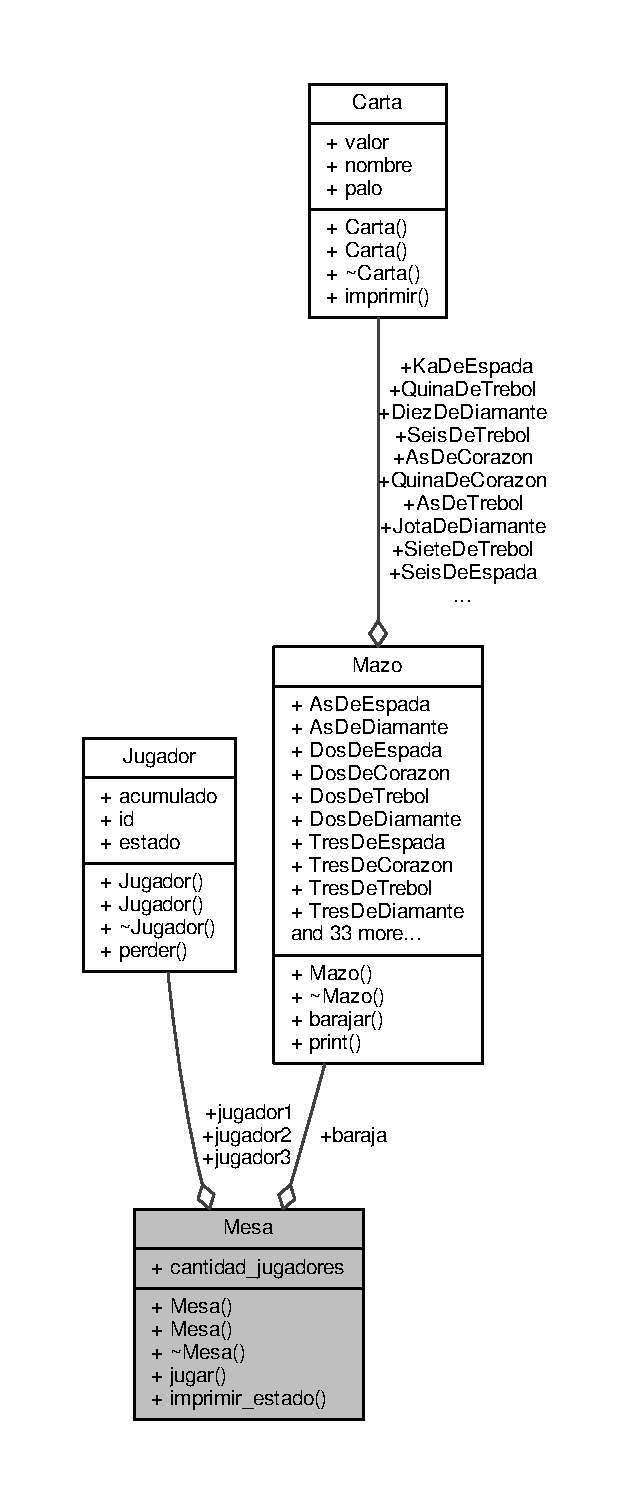
\includegraphics[height=550pt]{class_mesa__coll__graph}
\end{center}
\end{figure}
\subsection*{Public Member Functions}
\begin{DoxyCompactItemize}
\item 
\hypertarget{class_mesa_a98794038db53804cb4295480c96b2c20}{\hyperlink{class_mesa_a98794038db53804cb4295480c96b2c20}{Mesa} ()}\label{class_mesa_a98794038db53804cb4295480c96b2c20}

\begin{DoxyCompactList}\small\item\em Constructor vacío de \hyperlink{class_mesa}{Mesa}. \end{DoxyCompactList}\item 
\hypertarget{class_mesa_adea67ec335ba9969f2e10aa8f8b7832b}{\hyperlink{class_mesa_adea67ec335ba9969f2e10aa8f8b7832b}{Mesa} (\hyperlink{class_jugador}{Jugador} $\ast$J1, \hyperlink{class_jugador}{Jugador} $\ast$J2, \hyperlink{class_jugador}{Jugador} $\ast$J3, \hyperlink{class_mazo}{Mazo} M1)}\label{class_mesa_adea67ec335ba9969f2e10aa8f8b7832b}

\begin{DoxyCompactList}\small\item\em Contructor de \hyperlink{class_mesa}{Mesa}. \end{DoxyCompactList}\item 
\hypertarget{class_mesa_aa0a1b83b8058f80f4f27ec46cc5e9524}{virtual \hyperlink{class_mesa_aa0a1b83b8058f80f4f27ec46cc5e9524}{$\sim$\+Mesa} ()}\label{class_mesa_aa0a1b83b8058f80f4f27ec46cc5e9524}

\begin{DoxyCompactList}\small\item\em Destructor de \hyperlink{class_portero}{Portero}. \end{DoxyCompactList}\item 
void \hyperlink{class_mesa_a05491b7be2de02347201c6aa40daf905}{jugar} (\hyperlink{class_portero}{Portero} sala\+\_\+espera, \hyperlink{class_mesa}{Mesa} $\ast$M1, \hyperlink{class_mesa}{Mesa} $\ast$M2, \hyperlink{class_mesa}{Mesa} $\ast$M3)
\begin{DoxyCompactList}\small\item\em Función cuando un jugador pierde. \end{DoxyCompactList}\item 
\hypertarget{class_mesa_ad4fc44150615ca42473e205fd77e7a4a}{void {\bfseries imprimir\+\_\+estado} ()}\label{class_mesa_ad4fc44150615ca42473e205fd77e7a4a}

\end{DoxyCompactItemize}
\subsection*{Public Attributes}
\begin{DoxyCompactItemize}
\item 
\hypertarget{class_mesa_a2f46f7d92ea38a343f5f45969e7b2c36}{int \hyperlink{class_mesa_a2f46f7d92ea38a343f5f45969e7b2c36}{cantidad\+\_\+jugadores}}\label{class_mesa_a2f46f7d92ea38a343f5f45969e7b2c36}

\begin{DoxyCompactList}\small\item\em Atributos de \hyperlink{class_mesa}{Mesa}. \end{DoxyCompactList}\item 
\hypertarget{class_mesa_a3e88757b479e3cd42a5f9b3f73601baf}{\hyperlink{class_jugador}{Jugador} $\ast$ {\bfseries jugador1}}\label{class_mesa_a3e88757b479e3cd42a5f9b3f73601baf}

\item 
\hypertarget{class_mesa_a7878cb758a95b29491f8c2ac49d9fef4}{\hyperlink{class_jugador}{Jugador} $\ast$ {\bfseries jugador2}}\label{class_mesa_a7878cb758a95b29491f8c2ac49d9fef4}

\item 
\hypertarget{class_mesa_a4412964bcc1c6f6cf13ebbf28251887d}{\hyperlink{class_jugador}{Jugador} $\ast$ {\bfseries jugador3}}\label{class_mesa_a4412964bcc1c6f6cf13ebbf28251887d}

\item 
\hypertarget{class_mesa_ac8fcd5ce6a4507da84d54c2237dadb3d}{\hyperlink{class_mazo}{Mazo} {\bfseries baraja}}\label{class_mesa_ac8fcd5ce6a4507da84d54c2237dadb3d}

\end{DoxyCompactItemize}


\subsection{Member Function Documentation}
\hypertarget{class_mesa_a05491b7be2de02347201c6aa40daf905}{\index{Mesa@{Mesa}!jugar@{jugar}}
\index{jugar@{jugar}!Mesa@{Mesa}}
\subsubsection[{jugar}]{\setlength{\rightskip}{0pt plus 5cm}void Mesa\+::jugar (
\begin{DoxyParamCaption}
\item[{{\bf Portero}}]{sala\+\_\+espera, }
\item[{{\bf Mesa} $\ast$}]{M1, }
\item[{{\bf Mesa} $\ast$}]{M2, }
\item[{{\bf Mesa} $\ast$}]{M3}
\end{DoxyParamCaption}
)}}\label{class_mesa_a05491b7be2de02347201c6aa40daf905}


Función cuando un jugador pierde. 

Llenado de la mesa

Repartición de las cartas

Decisión de quién perdió

Repartición de las cartas

Decisión de quién perdió

Repartición de las cartas

Decisión de quién perdió 

The documentation for this class was generated from the following files\+:\begin{DoxyCompactItemize}
\item 
Mesa.\+h\item 
Mesa.\+cpp\end{DoxyCompactItemize}

\hypertarget{class_portero}{\section{Portero Class Reference}
\label{class_portero}\index{Portero@{Portero}}
}


Collaboration diagram for Portero\+:
\nopagebreak
\begin{figure}[H]
\begin{center}
\leavevmode
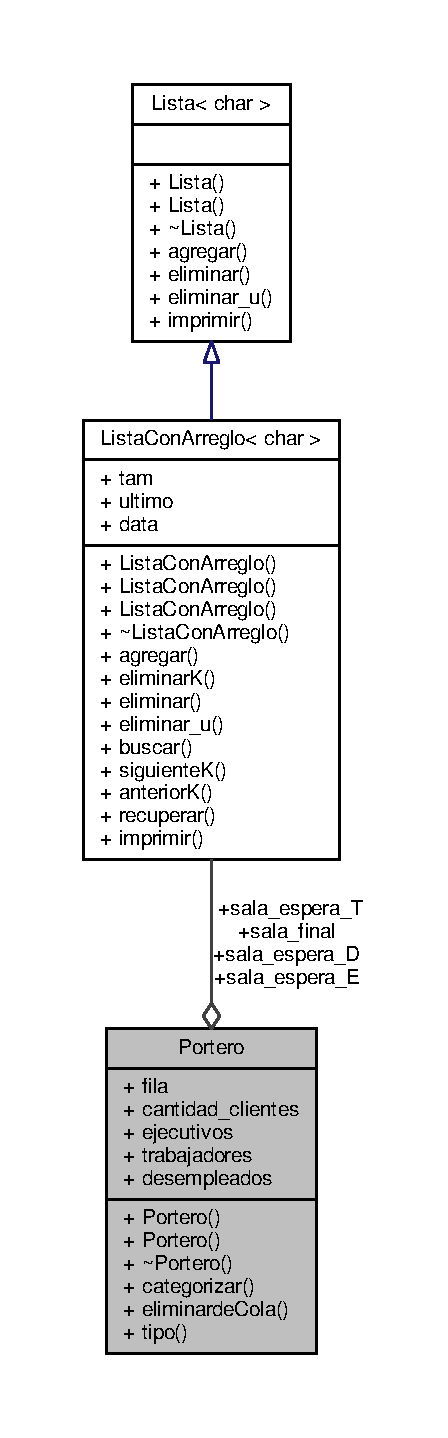
\includegraphics[height=550pt]{class_portero__coll__graph}
\end{center}
\end{figure}
\subsection*{Public Member Functions}
\begin{DoxyCompactItemize}
\item 
\hypertarget{class_portero_a7d760bc2477fe16dbb23c433a6aca4b2}{\hyperlink{class_portero_a7d760bc2477fe16dbb23c433a6aca4b2}{Portero} ()}\label{class_portero_a7d760bc2477fe16dbb23c433a6aca4b2}

\begin{DoxyCompactList}\small\item\em Contructor vacío de Porterno. \end{DoxyCompactList}\item 
\hypertarget{class_portero_a5534b8e4da1f89e0c84accd77afec404}{\hyperlink{class_portero_a5534b8e4da1f89e0c84accd77afec404}{Portero} (char $\ast$fila\+\_\+consola, int cantidad\+\_\+clientes, int ej, int tr, int de)}\label{class_portero_a5534b8e4da1f89e0c84accd77afec404}

\begin{DoxyCompactList}\small\item\em Contructor de \hyperlink{class_portero}{Portero}. \end{DoxyCompactList}\item 
\hypertarget{class_portero_a62e60c59b6211299f40e3cff5ba89ab2}{virtual \hyperlink{class_portero_a62e60c59b6211299f40e3cff5ba89ab2}{$\sim$\+Portero} ()}\label{class_portero_a62e60c59b6211299f40e3cff5ba89ab2}

\begin{DoxyCompactList}\small\item\em Destructor de \hyperlink{class_portero}{Portero}. \end{DoxyCompactList}\item 
\hypertarget{class_portero_a9887c6b1b6d710188e4c8d00bbd87282}{void \hyperlink{class_portero_a9887c6b1b6d710188e4c8d00bbd87282}{categorizar} ()}\label{class_portero_a9887c6b1b6d710188e4c8d00bbd87282}

\begin{DoxyCompactList}\small\item\em Función de agregar a sala de espera. \end{DoxyCompactList}\item 
\hypertarget{class_portero_ae4c80a71fc3f5aa0f2951770e5f68d0d}{void \hyperlink{class_portero_ae4c80a71fc3f5aa0f2951770e5f68d0d}{eliminarde\+Cola} ()}\label{class_portero_ae4c80a71fc3f5aa0f2951770e5f68d0d}

\begin{DoxyCompactList}\small\item\em Función de sacar de Cola/\+Sala/\+Casino. \end{DoxyCompactList}\item 
\hypertarget{class_portero_ac59d476839cdff7a231672a9b42b340f}{char {\bfseries tipo} (int k)}\label{class_portero_ac59d476839cdff7a231672a9b42b340f}

\end{DoxyCompactItemize}
\subsection*{Public Attributes}
\begin{DoxyCompactItemize}
\item 
\hypertarget{class_portero_af647147300727120b6c11c195923d79a}{char $\ast$ \hyperlink{class_portero_af647147300727120b6c11c195923d79a}{fila}}\label{class_portero_af647147300727120b6c11c195923d79a}

\begin{DoxyCompactList}\small\item\em Atributos del Potero. \end{DoxyCompactList}\item 
\hypertarget{class_portero_a379a422542277f39f9b4caf7ea9bdce8}{\hyperlink{class_lista_con_arreglo}{Lista\+Con\+Arreglo}$<$ char $>$ {\bfseries sala\+\_\+espera\+\_\+\+E}}\label{class_portero_a379a422542277f39f9b4caf7ea9bdce8}

\item 
\hypertarget{class_portero_a0f7243f7d491ed2dd7c2e2c1391ca3f3}{\hyperlink{class_lista_con_arreglo}{Lista\+Con\+Arreglo}$<$ char $>$ {\bfseries sala\+\_\+espera\+\_\+\+T}}\label{class_portero_a0f7243f7d491ed2dd7c2e2c1391ca3f3}

\item 
\hypertarget{class_portero_af639be54624551e0b057e5f61959d0a9}{\hyperlink{class_lista_con_arreglo}{Lista\+Con\+Arreglo}$<$ char $>$ {\bfseries sala\+\_\+espera\+\_\+\+D}}\label{class_portero_af639be54624551e0b057e5f61959d0a9}

\item 
\hypertarget{class_portero_a44df5db8f8efbbeb2ba2703b54b3818a}{\hyperlink{class_lista_con_arreglo}{Lista\+Con\+Arreglo}$<$ char $>$ {\bfseries sala\+\_\+final}}\label{class_portero_a44df5db8f8efbbeb2ba2703b54b3818a}

\item 
\hypertarget{class_portero_ae8b48dbbca5c00251b1a2434a8bbe4e3}{int {\bfseries cantidad\+\_\+clientes}}\label{class_portero_ae8b48dbbca5c00251b1a2434a8bbe4e3}

\item 
\hypertarget{class_portero_a219dc18f72eb4625b3038ddd51491e26}{int {\bfseries ejecutivos}}\label{class_portero_a219dc18f72eb4625b3038ddd51491e26}

\item 
\hypertarget{class_portero_a57f0dc04400c99f82db321ffc379d207}{int {\bfseries trabajadores}}\label{class_portero_a57f0dc04400c99f82db321ffc379d207}

\item 
\hypertarget{class_portero_ab247c04b02ac2034e32ffa4c43655cb7}{int {\bfseries desempleados}}\label{class_portero_ab247c04b02ac2034e32ffa4c43655cb7}

\end{DoxyCompactItemize}


The documentation for this class was generated from the following files\+:\begin{DoxyCompactItemize}
\item 
Portero.\+h\item 
Portero.\+cpp\end{DoxyCompactItemize}

%--- End generated contents ---

% Index
\newpage
\phantomsection
\addcontentsline{toc}{chapter}{Index}
\printindex

\end{document}
